\section{Operating Modes}

\subsection{Introduction}
The GPIO core supports bidirectional IO pads, and each IO can be programmed to operate in 
push-pull or open drain mode, as defined by te MODE register.

Note: IO Pads are not implemented within the GPIO core - this is the responsiblity of the designer

\subsection{Push-Pull Mode}
In this mode, each bit of gpioOutput is driven from the internal OUTPUT register. The gpioOutputEnable bus is controlled via the DIRECTION register and 
specifies whether or not the pin will allow the IO Pad to see the corresponding OUTPUT data.

\begin{figure}[h]
    \centering
    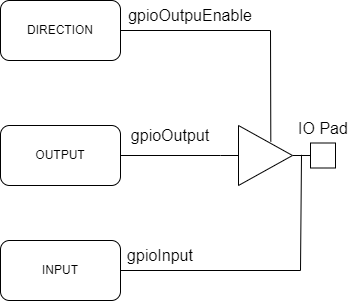
\includegraphics[width=0.4\textwidth]{images/ppl.png}
    \caption{Push Pull Mode}
  \end{figure}

\subsection{Open Drain Mode}
In this mode, each bit of gpioOutput is driven low when the corresponding OUTPUT register bit is low and corresponding DIRECTION register bit is high. 
This allows for multiple devices to pull the line low without conflicting high/low states on the output pin.

\begin{figure}[h]
    \centering
    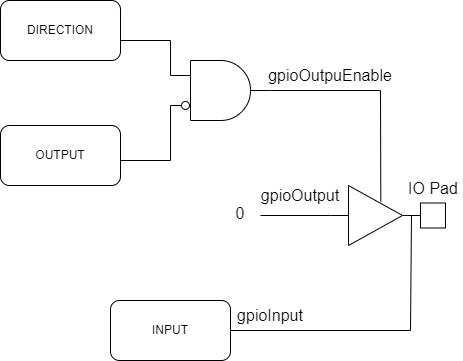
\includegraphics[width=0.4\textwidth]{images/od.drawio.png}
    \caption{Open Drain Mode}
  \end{figure}